\documentclass[border=10pt]{standalone}
\usepackage{tikz}\usepackage{amsmath}\usetikzlibrary{calc,arrows.meta}
\begin{document}
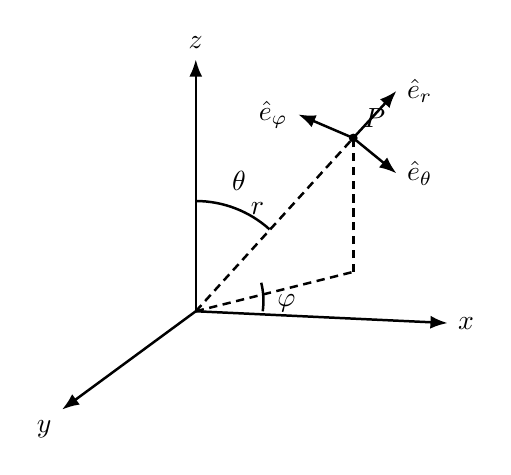
\begin{tikzpicture}[line width=0.9pt,>={Latex[length=2.2mm]}]
  \coordinate (O) at (0,0);
  \draw[->] (O)--(0,3.2) node[above]{$z$};
  \draw[->] (O)--(3.2,-0.15) node[right]{$x$};
  \draw[->] (O)--(-1.7,-1.25) node[below left]{$y$};
  \coordinate (P) at (2.0,2.2);
  \coordinate (Pp) at (2.0,0.5);
  \draw[densely dashed] (O)--(P) node[midway,above left]{$r$};
  \draw[densely dashed] (O)--(Pp); \draw[densely dashed] (Pp)--(P);
  \fill (P) circle(1.6pt) node[above right]{$P$};
  % theta desde z
  \draw (0,1.4) arc (90:48:1.4); \node at (0.55,1.65){$\theta$};
  % phi en el plano
  \draw (0.85,0) arc (-8:14:0.95); \node at (1.15,0.1){$\varphi$};
  \draw[->] (P)--($(P)+(0.55,0.6)$) node[right]{$\hat e_r$};
  \draw[->] (P)--($(P)+(0.55,-0.45)$) node[right]{$\hat e_\theta$};
  \draw[->] (P)--($(P)+(-0.7,0.3)$) node[left]{$\hat e_\varphi$};
\end{tikzpicture}
\end{document}
